\documentclass[a4paper,11pt]{article}

\usepackage{amsmath}
\usepackage{amssymb}

% for proofs  environment
\usepackage{amsthm}

\usepackage[backend=bibtex]{biblatex}
\bibliography{prob-set-3}

% for probability trees
\usepackage{tikz}
\usetikzlibrary{trees}

% for Venn diagrams
\usetikzlibrary{shapes,backgrounds}
% for plots
\usepackage{ pgfplots}
% inserted on suggestion in warning during compilation
\pgfplotsset{compat=1.9}

%for strikethrough text
\usepackage{soul}

%for R source code listing
\usepackage{listings}

%for block quotes
\usepackage{csquotes}

% For not indenting the first line of paragraphs:
\setlength{\parindent}{0pt}
% define the title
\author{John Hancock}
\title{MIT Introduction to Statistics 18.05 Problem Set 3 }
\begin{document}
% generates the title
\maketitle
% insert the table of contents
\tableofcontents
\section{References and License}
We are answering questions in the material from MIT OpenCourseWare
course 18.05, Introduction to Probability and Statistics.

In this document we are answering questions Orloff and Bloom ask in
\cite{probSet3}.

Please see the references section for detailed citation information.

The material for the course is licensed under the terms at
\url{http://ocw.mit.edu/terms}.

We use documentation in \cite{vennDiagram}, \cite{nodePos}, \cite{plotPoints},
\cite{plotFunc} to write \LaTeX source code for this document.
\section{Independence}

In this section we answer a problem in \cite{probSet3} that involves rolling
two six sided dice.

\subsection{Pairwise and mutual independence}
We define two events, $A$, and $B$ to be pairwise independent if
$P \left( A \cap B \right) = P \left( A \right) P \left(B \right)$.

For this problem Orloff and Bloom give us the definition of mutual independence
for three events, $A$, $B$, and $C$.  $A$, $B$, and $C$ are mutally independent
if
\begin{equation}
	P \left( A \cap B \cap C\right)
	= P \left(A \right) P \left(B \right) P \left( C \right)
\end{equation}

In this section, Orloff and Bloom give the following definitions for events
$A$, $B$, and $C$:
\begin{itemize}
	\item $A$ is the event that we roll an odd number with the first die.
	\item $B$ is the event that we roll an odd number with the second die.
	\item $C$ is the event that the sum of the numbers we roll is odd.
\end{itemize}

$A$, $B$, and $C$ are not mutually independent.  Whatever the
$A$, $B$, and $C$ probabilities of $A$, $B$, and $C$ are individually, the
probability of  $P \left( A \cap B \cap C\right)$ is $0$ since the sum of two
odd numbers is always an even number.

\subsection{Venn diagram}

Orloff and Bloom give the following Venn diagram:

\def\firstcircle{(0,0) circle (1.5cm)}
\def\secondcircle{(45:2cm) circle (1.5cm)}
\def\thirdcircle{(0:2cm) circle (1.5cm)}

\begin{center}
\begin{tikzpicture}
\begin{scope}[shift={(3cm,-5cm)}, fill opacity=0.3]
        \fill[red] \firstcircle;
        \fill[green] \secondcircle;
        \fill[blue] \thirdcircle;
        \draw \firstcircle node[below, opacity=1] {$0.225$} node[xshift=1cm, yshift=0.3cm, opacity=1] {$0.125$} node[left, yshift=0.5cm, opacity=1] {$A$};
        \draw \secondcircle node [above, opacity=1] {$0.225$}
				%intersection of a and b below:
					node[below, xshift=0.6cm, yshift=-0.2cm, opacity=1]{$0.1$}
				%intersection of b and c below:
					node[below, xshift=-1.1cm, opacity=1]{$0.05$}
					node[left, yshift=0.7cm, opacity=1] {$B$};
        \draw \thirdcircle node [below, opacity=1] {$0.175$}
					node[left, xshift=-0.6cm, yshift=-0.5cm, opacity=1]{$0.1$}
					node[left, xshift=1.2cm, yshift=0cm, opacity=1] {$C$};
					node[xshift=]
    \end{scope}
\end{tikzpicture}
\end{center}

And ask us whether or not the events in the Venn diagram above are mutually
independent.

These events are not mutually independent because
\begin{equation}
	P \left(A \right) P \left(B \right) P \left( C \right) =
		0.225 \times 0.225 \times 0.175 = 0.008859375.
\end{equation}

However, in the Venn diagram above, Orloff and Bloom give us that
$P \left( A \cap B \cap C\right) = 0.125$

Therefore the events are not mutually independent.

\subsection{How many kids}
For this question we use the same assumptions about the probability of the
gender that a child is born with that Orloff and Bloom use in example 9 of
\cite{reading4a}.

We define the following events:

\begin{itemize}
\item $A$ is the event that the children in a family are both boys and girls.
\item $B$ is the event that at most one of the children is a girl.
\item $C_{i,b}$ is the event that child number $i$ is a boy.
\item $C_{i,g}$ is the event that child number $i$ is a girl.
\end{itemize}

Our goal is to construct a sample space such that $A$ and $B$ are independent.
The definition of independent events is in \cite{reading3}.

We rely on the same assumption that Orloff and Bloom make in \cite{reading4a}
regarding the probability of the genders of sequences of children.

Therefore we assume  $P\left( C_{i,b} \right) = 0.5$, and $P\left( C_{i,g} \right) = 0.5$,
independent of the event that any other child is a boy or a girl.

We write the following table to discover the number of children where
$A$, and $B$ will meet the definition of independent events.

We fill in one cell in the table below for each possible
sequnce of three children in the family being boys
or girls.

\begin{center}
  \begin{tabular}{ | c | c | c | c | }
    \hline
	$C_{1,b}C_{2,b}C_{3,b}$ & $C_{1,b}C_{2,b}C_{3,g}$ & $C_{1,b}C_{2,g}C_{3,b}$ & $C_{1,b}C_{2,g}C_{3,g}$   \\ \hline
  $C_{1,g}C_{2,b}C_{3,b}$ & $C_{1,g}C_{2,b}C_{3,g}$ & $C_{1,g}C_{2,g}C_{3,b}$ & $C_{1,g}C_{2,g}C_{3,g}$   \\ \hline
  \end{tabular}
\end{center}

In the table above there are $6$ sequences that are in $A$, so $P\left( A \right) = \frac{6}{8}$.

Also, there are $4$ sequences in $B$, so $P\left( B \right) = \frac{4}{8}$.

Moreover, there are $3$ sequences where there is at most one girl, and
the children are both boys and girls.  Therefore $P\left( A \cap B \right) = \frac{3}{8}$.

$A$ and $B$ are indpendent since
\begin{equation}
P\left(A \right) P \left( B \right)
  = \left( \frac{6}{8} \right) \left( \frac{4}{8} \right)
  = \frac{24}{64} = \frac{3}{8}.
\end{equation}

Therefore $P\left(A \right) P\left(B \right) = P \left(A \cap B \right)$,
so $A$ and $B$ must be independent events.

We made these calculations assuming that there are $3$ children,
therefore the number of children we require in order for $A$, and
$B$ to be independent events is $3$.

\section{R simulation}

Note: we needed to refer to \cite{rStandardDev} to recall the R function for
standard deviation.

\subsection{Mean and standard deviation}

We use R functions to compute the mean and standard deviation of the data
that Orloff and Bloom give us for this problem:

\begin{lstlisting}
> mean(x)
[1] 2.554528
> sd(x)
[1] 2.07408
\end{lstlisting}

\subsection{Histogram of the data}

We rely on the examples in \cite{studio3} in order to write the R code to
produce the histogram Orloff and Bloom require.

The R code is
\begin{lstlisting}
binwidth = .1
bins = seq(min(x), max(x)+binwidth, binwidth)
hist(x, breaks=bins, col='yellow', freq=TRUE)
\end{lstlisting}

The histogram this code produces is:

\begin{center}
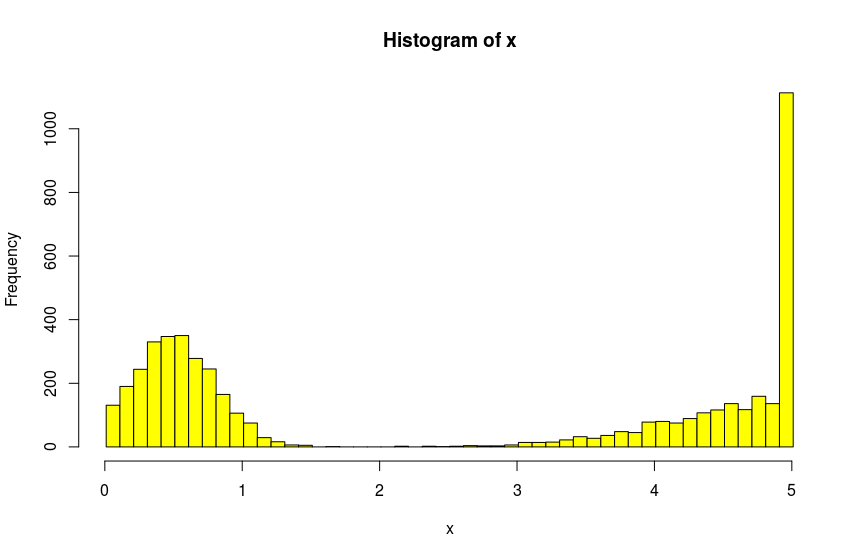
\includegraphics[scale=0.5]{histogram-prob2}
\end{center}

\subsection{Conclusions on the data}
The mean value of the data that we use R to compute above tells us that
the mean number of years a patient lives after receiving the treatment is
approximately $2.555$ years.  However, the standard deviation we compute
using R tells us that the spread of values in the data is approximately
$\frac{4}{5}$ of the mean number of years that a patient is expected to live
after receiving the treatment.  That means that we have many values in the
data that are larger and smaller than the mean value of the data. The histogram
we plot bears this out; we see taller bins on the left and
right hand sides of the histogram.

\subsection{Effectiveness of the treatment}
The tallest bin is on the right hand side of the histogram.  To us, this implies
that for some patients, the treatment is effective.  We would recommend
research to determine what thing or things the patients whose data lies in
the rightmost bins have in common.  Furthermore we would recommend that we
conduct experiments to determine which of the things these patients have in
common is or are the thing(s) that implies or imply the treatment is effective.

\section{Dice}

In this section we will deal with problems that Orloff and
Bloom ask about the random variable $X$, that is equal to the value
we roll with a fair $4$-sided die, the random variable
$Y$, that is equal to the value we roll with a fair $6$ sided die,
and the random variable $Z$, that is equal to the average
of $X$ and $Y$.

\subsection{Standard deviation of $X$, $Y$, and $Z$}


We use the definition of variance and standard deviation in \cite{reading5a} to
calculate the standard deviations $\sigma \left( X \right)$, $\sigma \left( Y \right)$.

We use the exact same method to calculate the variance of a discrete random
variable many times. For details on how to do the calculation see
\cite{reading5aAns}.  We calculate the variance of $X$, and $Y$, then take
the square root of the variance to obtain the standard deviation.

Here are the results:

\begin{equation}
  \sigma_{X} \approx 1.118.
\end{equation}

\begin{equation}
	\sigma_{Y} \approx 1.708.
\end{equation}

In order to calculate the variance of $Z$, we can use properties of variance
that Orloff and Bloom show in \cite{reading5a}.

$X$ and $Y$ are independent random variables; the value we roll with a fair four
sided die has no effect on the value we roll with a fair six sided die.
Therefore the equation
\begin{equation}
	\text{Var}\left(X + Y \right)
	= \text{Var}\left(X \right) + \text{Var}\left( Y \right).
\end{equation}

We will also use the property of variance Orloff and Bloom show in
\cite{reading5a} that
\begin{equation}
	\text{Var}\left(X \right) = a^{2}\text{Var}\left(X \right).
\end{equation}

Therefore, in the scope of this problem,
\begin{equation}
	\text{Var} \left(\frac{X+Y}{2} \right)
		= \text{Var}\left( \frac{X}{2} + \frac{Y}{2} \right)
		= \frac{1}{4} \left( \text{Var}\left( X \right)
			+ \text{Var}\left( Y \right)\right).
\end{equation}

We use the values we calculated for $\text{Var}\left(X \right)$, and
$\text{Var}\left(Y \right)$ above,
\begin{equation}
	\text{Var}\left(Z \right) \approx \frac{1}{4}\left(1.118 + 1.708 \right)
		\approx 0.707
\end{equation}

Standard deviation is the square root of variance, so
\begin{equation}
	\sigma_{z} \approx \sqrt{\frac{1}{4}\left(1.118^{2} + 1.708^{2} \right)}
		\approx 1.021
\end{equation}

\subsection{Graph pmf and cdf of $Z$}

We use R to simulate rolling the dice.  We find documentation in \cite{rTable}
helpful in writing this source code.  Here is a listing of the R source
code:
\begin{lstlisting}
y=sample(c(1:6), replace = TRUE, 1000000)
x=sample(c(1:4), replace = TRUE, 1000000)
z=(x+y)/2
zTable = table(z)
zTable/1000000
\end{lstlisting}

The output of this program is:
\begin{lstlisting}
	z
       1      1.5        2      2.5        3
0.041375 0.083538 0.125244 0.167014 0.166669
3.5        4      4.5        5
0.167029 0.124364 0.083153 0.041614
\end{lstlisting}

Note: we edit the output of the program so that the output is visible.

We look at the numerical inverses of the values in the second row of the
table above to get a clue about the probability mass of each possible value
of $Z$.  Here again we utilize R to compute the inverses:

\begin{lstlisting}
freqs=c(0.041375, 0.083538, 0.125244, 0.167014, 0.166669,
0.167029, 0.124364, 0.083153, 0.041614 )
1/freqs
\end{lstlisting}

Note: we added a line break to the listing above so that the listing is
visible.

We execute the code above to get the result
\begin{lstlisting}
24.169184 11.970600  7.984414  5.987522  5.999916
5.986984  8.040912 12.026024 24.030374
\end{lstlisting}

Note: we added a line break to the listing above so that the output is visible.

Now it becomes clear that we can approximate the frequencies of the values of
$Z$ as fractions with $24$ in the denominator.  We summarize this approximation
in the table below, and make a guess as to the value of the pmf of $Z$:

\begin{center}
  \begin{tabular}{ | c | c | c | c | c | c | c | c | c | c |}
    \hline
	$Z$ & 1 & 1.5 & 2 & 2.5 & 3 & 3.5 & 4 & 4.5 & 5  \\ \hline
  pmf $p\left( z \right)$ ? & $\frac{1}{24}$ & $\frac{2}{24}$ & $\frac{3}{24}$ &
		$\frac{4}{24}$ & $\frac{4}{24}$ & $\frac{4}{24}$ & $\frac{3}{24}$ & $\frac{2}{24}$ &
		$\frac{1}{24}$ \\ \hline
  \end{tabular}
\end{center}
The data from the sumulation inspires us to make the following reasoning about
the pmf of $Z$:  There are $6 \times 4$ possible pairs of values we can roll
with the two dice.  To compute the value of $Z$ we add the pair of values, and
divide by $2$.  Some of the values of $Z$ will occur more frequently because
there are more values of $X$ and $Y$ divided by $2$ that equal a particular
value of $Z$.  $1.5=\frac{1+2}{2}$, and $1.5=\frac{2+1}{2}$.  The order of
terms in the sum is important because the first number is the value we roll
with the $4$-sided die, and the second number is the value we roll with the
$6$-sided die.  $2=\frac{1+3}{2}=\frac{2+2}{2}=\frac{3+1}{2}$.
$2.5=\frac{1+4}{2}=\frac{2+3}{2}=\frac{3+2}{2}=\frac{4+1}{2}$.
$3=\frac{1+5}{2}=\frac{2+4}{2}=\frac{3+3}{2}=\frac{4+2}{2}$.
$3.5=\frac{1+6}{2}=\frac{2+5}{2}=\frac{3+4}{2}=\frac{4+3}{2}$.
$4=\frac{2+6}{2}=\frac{3+5}{2}=\frac{4+4}{2}$.
$4.5=\frac{3+6}{2}=\frac{4+5}{2}$
$5=\frac{4+6}{2}$.  Hence the pmf for a particular value of $Z$ is the number
of ways of summing a value between $1$ and $4$, and a value between $1$ and
$6$, and dividing by $2$ to equal $Z$.

Therefore the tentative pmf we write in the table above is the pmf for $Z$.

Here is a plot of the pmf:
\begin{center}
 \begin{tikzpicture}[x=1cm,y=2cm]


 \draw[latex-latex, thin, draw=gray] (0,0)--(6,0) node [right] {$x$}; % l'axe des abscisses
 \draw[latex-latex, thin, draw=gray] (0,0)--(0,1) node [above] {$y$}; % l'axe des ordonnées

\foreach \Point in {(1, 0.0417), (1.5, 0.08333), (2, 0.125), (2.5, 0.16667), (3, 0.16667),
	(3.5, 0.166667), (4, 0.125), (4.5, 0.08333), (5, 0.0417)}{
    \node at \Point {\textbullet};
}

% to ensure that the points are being properly centered:
\draw [dotted, gray] (0,0) grid (6,1);

\end{tikzpicture}
\end{center}

Orloff and Bloom ask for a plot of the of the cumulative distribution function
(CDF) of $Z$.

Orloff and Bloom define and explain how to calculate the CDF in
\cite{reading4a}.

Here is a plot of the cdf of $Z$:
\begin{center}
 \begin{tikzpicture}[x=1cm,y=2cm]


 \draw[latex-latex, thin, draw=gray] (0,0)--(6,0) node [right] {$x$}; % l'axe des abscisses
 \draw[latex-latex, thin, draw=gray] (0,0)--(0,1) node [above] {$y$}; % l'axe des ordonnées

\foreach \Point in {(1, 0.0417), (1.5, 0.12503), (2, 0.25003), (2.5, 0.417), (3, 0.583),
	(3.5, 0.75), (4, 0.875), (4.5, 0.958), (5, 1.0)}{
    \node at \Point {\textbullet};
}
% to ensure that the points are being properly centered:
\draw [dotted, gray] (0,0) grid (6,1);
\end{tikzpicture}
\end{center}

\subsection{Game}

In this section we answer the quesion Orloff and Bloom pose regarding a game
where we win $2X$ dollars if $X > Y$ and we lose $1$ dollar otherwise.

They ask us after playing the game $60$ times, what is our expected total gain
or loss.

In order to answer, we need to know the probability $P \left(X > Y \right)$.

We wrote the following R simulation to get an idea of what
$P \left(X > Y \right)$ is.

\begin{lstlisting}
winCount=0
loseCount=0
for ( i in 1:100000){
  x=sample(c(1:4), replace=TRUE, 1)
  y=sample(c(1:6), replace=TRUE, 1)
  if (x > y){
    winCount = winCount + 1
  } else{
    loseCount = loseCount + 1
  }
}
print(winCount/1000);
\end{lstlisting}

The output of this simulation is close to 0.25 every time we run it, so
we should be able to find a reason why $P \left(X > Y \right) = 0.25$.

These are the possible combinations of values we can roll with a $6$-sided
die, and a $4$-sided die. We deonte a pair of values where we win with a
$W$, and a pair of values where we loose with an $L$.

The first value in each pair is the value we roll with the $4$-sided die, and
the second value in each pair is the value we roll with the $6$-sided die.

$1, 1 L$, $2, 1 W$, $3, 1 W$, $4, 1 W$

$1 ,2 L$, $2, 2 L$, $3, 2 W$, $4, 2 W$

$1 ,3 L$, $2, 3 L$, $3, 3 L$, $4, 3 W$

$1 ,4 L$, $2, 4 L$, $3, 4 L$, $4, 4 L$

$1 ,5 L$, $2, 5 L$, $3, 5 L$, $4, 5 L$

$1 ,6 L$, $2, 6 L$, $3, 6 L$, $4, 6 L$

Now, to calculate the probability that $X > Y$, we count the number of $W$'s
above, and divide by the sum of the number of $W$'s and $L$'s.

There are $6$ $W$'s  and $24$ $W$'s and $L$'s, so the probability that
$X > Y$ is $\frac{6}{24} = \frac{1}{4}$.

We calculate the expected number of dollars we win or lose playing one round
of the game, then multiply that number by 60 to compute our expceted profit
or loss playing 60 rounds of the game.

We define $W$ as the event that we win. $P\left( W \right)$ is the probability
of winning one round of the game, and $1-P\left( W \right)$ is the probability
of losing one round of the game. Then by what we show immediately above,
$P\left( W \right) = \frac{1}{4}$.

We introduce two new discrete random variables:
\begin{itemize}
	\item $X^{\prime}$: the number of dollars we win playing one round of the
		game.
	\item $Y^{\prime}$: the number of dollars we lose plaing one round of the
		game.
\end{itemize}

We define a third random variable $W^{\prime}$ to be  $X^{\prime}-Y^{\prime}$.
$W^{\prime}$ is the number of dollars we win or lose playing one round of the
game.

Now we can use the definition of expected value \cite{reading4a} to obtain the
expected value of our profit or loss playing the game.

\begin{equation} \label{expectedW}
E \left( W^{\prime} \right) = P\left( W \right) E \left( X^{\prime} \right)
	- \left( 1 - P \left(W \right)\right) E \left(Y^{\prime} \right)
\end{equation}

Now we consider how to calculate $E\left( X^{\prime} \right)$.  We show above that
we have a $\frac{1}{4}$ probability of winning the game.  We remind the reader
that Orloff and Bloom give us that we are playing with fair dice in this
problem. We show in the listing of possible outcomes of the game above that
there are $6$ outcomes where we win.  Since the dice are fair, each of the
$6$ outcomes are equally likely, but we win the same number of dollars
for some of the outcomes.  So the expected number of dollars we can win
playing one round of the game is:
\begin{equation}
	\frac{4+6+6+8+8+8}{6}=\frac{40}{6}=6\frac{2}{3}.
\end{equation}

According to the rules of the game that Orloff and Bloom give, the expected
number of dollars we can lose playing one round of the game is $1$ dollar.

Now we have values for all of the quantities on the right hand side of
equation \ref{expectedW}.  Hence

\begin{equation}
E \left( W^{\prime} \right) = \frac{1}{4}\times \$ 6 \frac{2}{3} -
	\left( 1 - \frac{1}{4} \right) \times \$ 1
	\approx \$0.917.
\end{equation}

Therefore, if we play $60$ rounds of the game, we expect to win approximately
$60 \times \$0.917 = \$55.02$.

\section{Two scoops}

In this section we answer questions Orloff and Bloom ask about raisins randomly
strewn throughout the volume of a box of cereal.

\subsection{Number of raisins in the box}
In order to cacluate the number of raisins in the box, we integrate the function
for the denisty of raisins in the box over the interval of the height of the
box. Orloff and Bloom give us that the height of the box is $30$ cm, and the
formula for the density of raisins in the box at height $h$ is,
$f \left( x \right) = 40 -h $

We define $R$ to be the number of raisins in the box. Then,
\begin{equation}
	R = \int_{0}^{30} 40 -h \text{ } dh.
\end{equation}

We use the power rule for integrals \cite{basicInt} to replace the integral
in the equation above with its anti-derivative:

\begin{equation}
	R = 40h - \frac{h^{2}}{2} \bigg\rvert_{0}^{h}.
\end{equation}

Orloff and Bloom state that the box is 30 cm tall, so the interval that we
are integrating over is $\left[0, 30 \right]$.  Therefore the number of raisins
in the box is:

\begin{equation}
	R = 40h - \frac{h^{2}}{2} \bigg\rvert_{0}^{30}
	= 40 \times 30 - \frac{30^{2}}{2} = 1200 - \frac{900}{2} = 1200 - 450 = 750.
\end{equation}

\subsection{PDF for height of random raisin}

In this section, Orloff and Bloom define $H$ to be the height of a random
raisin, and $g \left( h \right)$ as the probability density function (PDF) of
$H$.  They ask us to graph $g \left( h \right)$.

First of all, we need a formula for $g$ that provides a function we can
integrate.  We know that the function for the density of raisins at height
$h$ is $40 - h$.

We use the anti-derivative of the raisin density function evaluated over
the interval $\left[ 0, h \right]$, $40h - \frac{h^{2}}{2} \bigg\rvert_{0}^{h}$
to compute the number of raisins in the volume of the box at or below height
$h$.

Orloff and Bloom define $H$ to be the height of a random raisin.  It is
appropriate for us to refine the definition of $H$.  We define $H$ as the
height of a raisin in the box, where we have chosen the raisin randomly from
the set of raisins in the box.

The notion of probability $P \left( H \right)$ that we associate with $H$ is the
probability that a raisin we choose randomly from the set of raisins in the box
is in the volume of the box at height h.

Then, the probability that a raisin we choose at random  is in the volume of the
box at height $h$ is the number of raisins in the box at height $h$, divided by
the total number of raisins in the box.

We know from what we calculated above that the total number of raisins in
the box is $750$.

Therefore the formula for the probability that a raisin chosen at random from
the set of raisins in the box is at height $h$ is
\begin{equation} \label{raisinProb}
	P\left( H \right)
 = \frac{1}{750} \left( 40h - \frac{h^{2}}{2} \bigg\rvert_{0}^{h} \right).
\end{equation}

Orloff and Bloom ask for the probability density function of $H$.  We can
take the first derivative of equation \ref{raisinProb} with respect to $h$ to
get a probability density function, $g \left( h \right)$ for $H$:

\begin{equation}
	g\left( h \right) =
	\frac{1}{750} \left( 40 - h \right).
\end{equation}

Orloff and Bloom require a plot of $g \left( h \right)$. Note: due to the very
small scale of $Y$ values, we do not draw the graph below to scale.

\begin{center}
\begin{tikzpicture}
      \draw[->] (0,0) -- (6, 0) node[right] {$h$};
      \draw[->] (0,0) -- (0,2) node[above] {$g \left(h \right)$};
      \draw[scale=1,domain=0:3.5,smooth,variable=\x,black] plot ({\x}, {1.75 - 0.5*\x});
			\draw [dotted, gray] (0,0) grid (6,2);
			\node at (-0.5, 1.75) {$\frac{40}{750}$};
			\node at (3.5, -.5) {$40$};
\end{tikzpicture}
\end{center}

\subsection{CDF of random raisin}

Orloff and Bloom ask us to find, and plot the cumulative distribution function
(CDF), $G \left( H \right)$.

In our reasoning on the precise meaning of the probabiltiy of the height of
a random raisin in the previous section, we found the cumulative distribution
function $G \left( H \right)$. $G \left( H \right)$ is equation
\ref{raisinProb}, evaluated over the interval $\left[0, h \right]$.

Since
\begin{equation}
	G\left( H \right)
 = \frac{1}{750} \left( 40h - \frac{h^{2}}{2} \bigg\rvert_{0}^{h} \right).
\end{equation}

When we evaluate $G$ over the interval $\left[ 0, h \right]$, the terms of $G$
that we bind to the value $0$ are equal to 0, so we We can simplify the formula
for $G \left( H \right)$:

\begin{equation}
	G\left( H \right)
 = \frac{1}{750} \left( 40h - \frac{h^{2}}{2}  \right).
\end{equation}


\begin{center}
\begin{tikzpicture}
      \draw[->] (0,0) -- (6, 0) node[right] {$h$};
      \draw[->] (0,0) -- (0,2) node[above] {$G \left(h \right)$};
      \draw[scale=1,domain=0:3,smooth,variable=\x,black] plot ({\x}, {(2/3)*\x - (1/9)*(\x*\x)});
      \draw[scale=1,domain=3:6,smooth,variable=\x,black] plot ({\x}, {1});
			\draw [dotted, gray] (0,0) grid (6,2);
			\node at (-0.5, 1) {$1$};
			\node at (3, -.5) {$30$};
\end{tikzpicture}
\end{center}

\subsection{Raisin in bottom third of box}

The probability that a raisin is in the bottom third of the box is $G(H)$
evaluated over the interval $\left[ 0, 10 \right]$, because the box is $30$cm
tall.

Therefore the probability is
$\frac{1}{750} \left( 40 \times 10 - \frac{10^{2}}{2}  \right)$. This
evaluates to $\frac{350}{750}$, which simplifies to
$\frac{7}{15} \approx 0.467$.

\section{The new normal}
In this section we investigate properties of the normal distribution.  We
apply properties of variance and standard deviation Orloff and Bloom
show in \cite{reading5b}.

\subsection{Mean and variance of $X$} \label{meanVarX}
Orloff and Bloom define a continuous random variable $X$ in terms of another
continuous random variable $Z$, where $Z \sim N \left(0, 1 \right)$.

Orloff and Bloom give us that $X = aZ + b$.

In \cite{reading5d} Orloff and Bloom state that, for continuous random
variables, $X$, and $Y$, if $Y = aX + b$, then
$text{Var}\left(Y \right) = a^{2}\text{Var}\left(X \right)$, and
$E \left( Y \right) = aE\left(X \right) + b$.
Since we are given that $X = aZ + b$, we know
$\text{Var}\left(X \right) = a^{2}\text{Var} \left( Z \right)$, and
$E\left(X \right) = aE\left(Z \right)+b$.  Because expected value and mean
have the same meaning in this course, if the mean value of $Z$ is $\mu$,
then the mean value of $X$ is $a\mu+b$.

\subsection{PDF of X} \label{pdfX}

We go to the definition of $F_x \left( x \right)$ in terms of probability.

\begin{equation}
F_x \left( x \right) = P \left( X leq x \right).
\end{equation}

$X = aZ + b$, so

\begin{equation}
	P \left( X \leq x \right) =
	P \left( aZ + b \leq x \right).
\end{equation}

We solve this inequality for $Z$:

\begin{equation}
	P \left( aZ + b \leq x \right) =
	P \left( Z \leq \frac{x-b}{a} \right).
\end{equation}

Now we can apply the definition of $\Phi \left( z \right)$ to the equation
above:

\begin{equation}
	P \left( Z \leq \frac{x-b}{a} \right) =
		\Phi \left( \frac{x-b}{a} \right)
\end{equation}


We use the chain rule that is the result of theorem 4.4.1 in \cite{chainRule}.

The chain rule states that if

\begin{equation}
	h\left( x \right) =
		f\left( g ( \left( x \right) \right),
\end{equation}

then

\begin{equation}
	h^{\prime}\left(x \right)
		= f^{\prime}\left( g \left( x \right)\right) g^{\prime} \left( x \right)
\end{equation}


We let $h \left( x \right) = \Phi \left( \frac{x-b}{a}) \right)$.

Then, by the chain rule:

\begin{equation}
	\Phi^{\prime} \left( \frac{x-b}{a} \right) =
		\phi \left( \frac{x-b}{a} \right) \left(\frac{1}{a} \right)
\end{equation}

We use the definition of $\phi$:

\begin{equation} \label{messyE}
		\phi \left( \frac{x-b}{a} \right) \left(\frac{1}{a} \right) =
	\frac{1}{\sqrt{2 \pi }} e^{\frac{ \left( \frac{ x-b }{a} \right)^{2}}{2}} \left(\frac{1}{a} \right).
\end{equation}

Note that:
\begin{equation}
\frac{ \left( \frac{ x-b }{a} \right)^{2}}{2} =
	\frac { \frac{ \left( x - b \right)^{2}} {a^2}}{2}
	= \frac{ \left( x -b \right)^2}{2a^2}.
\end{equation}
Now we can simplify the right hand side of equation \ref{messyE}:

\begin{equation}
	\frac{1}{\sqrt{2 \pi }} e^{\frac{ \left( \frac{ x-b }{a} \right)^{2}}{2}} \left(\frac{1}{a} \right).
	= \frac{1}{a \sqrt{2 \pi }} e^{\frac{ \left( x-b \right)^{2}}{2a^2}}.
\end{equation}

Therefore the the PDF of $X$ is
\begin{equation} \label{pdfX}
 f_{X} \left( x \right)
	= \frac{1}{a \sqrt{2 \pi }} e^{\frac{ \left( x-b \right)^{2}}{2a}}.
\end{equation}

\subsection{$X$ follows $N \left( b, a^{2} \right)$} \label{prob5c}

Let $\mu=b$, and $\sigma=a^2$ then we use the definition of
$\phi \left( \mu, \sigma \right)$:

\begin{equation}
\frac{1}{\sigma \sqrt{2 \pi }} e^{\frac{ \left( x - \mu \right)^{2}} {2 \sigma^{2}}}
= \frac{1}{a \sqrt{2 \pi }} e^{\frac{ \left( x - b \right)^{2}} {2 a^{2}}}.
\end{equation}

The right hand side of the equation above is the same as the right hand side of
equation \ref{pdfX}, therefore $X \sim N \left( b, a^2 \right)$.

\subsection{$N \left( \mu, \sigma \right)$ mean and variance}

\section{Birth day}

In this problem, Orloff and Bloom give us that human gestation is approximated
with a normal distribution with mean $280$ days and a standard deviation of
$8.5$ days.

\subsection{Plots of PDF and CDF }

Note: we rely on documentation in \cite{plotTitle} to write the R code
below, as well as the example code in \ref{studio3}.

We write the following R code to produce a plot of the PDF of human gestation:

\begin{lstlisting}
z = seq(0,320,1)
plot(z,dnorm(z,280,8.5), type='l', col='blue', lwd=3)
title(main='PDF')
\end{lstlisting}

Here is the resulting plot:
\begin{center}
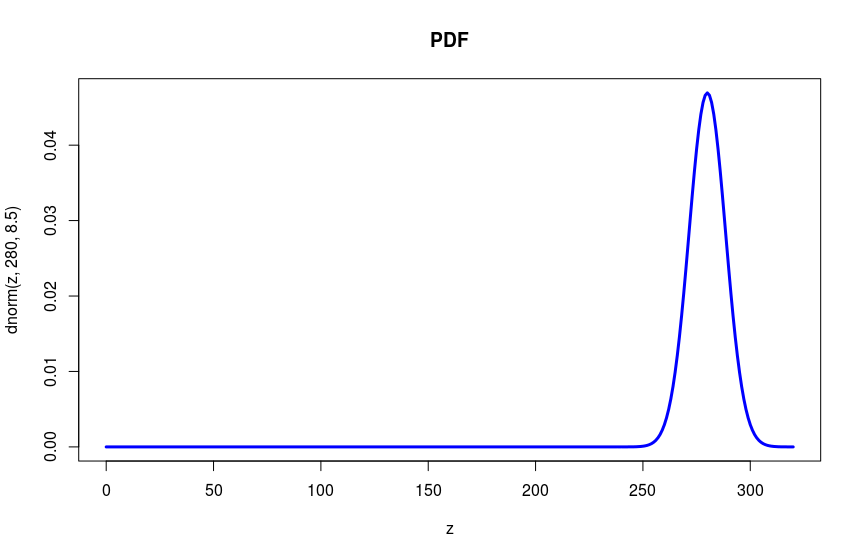
\includegraphics[scale=0.5]{pdf-gestation}
\end{center}

We write the following R code to produce a plot of the CDF of human gestation:

\begin{lstlisting}
z = seq(0,320,1)
plot(z, pnorm(z, 280, 8.5), type='l', col='red', lwd=3)
title(main='CDF')
\end{lstlisting}

Here is the resulting plot:
\begin{center}
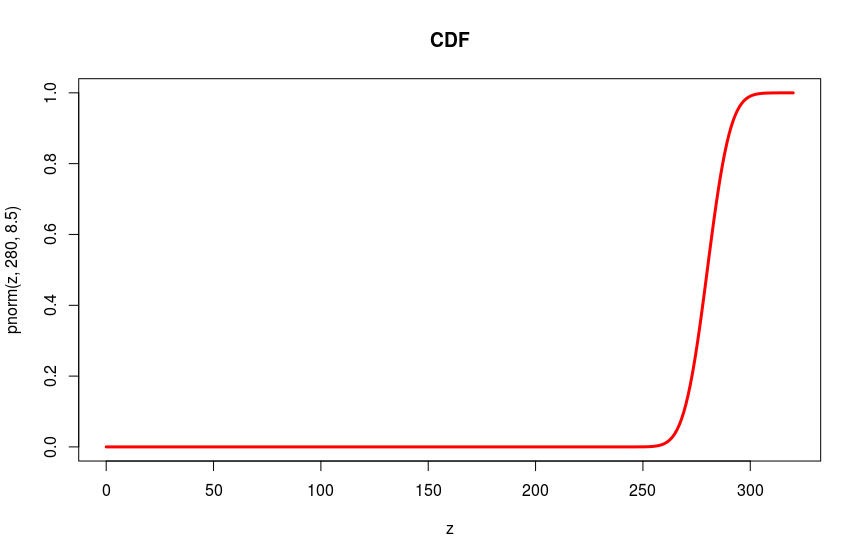
\includegraphics[scale=0.5]{cdf-gestation}
\end{center}

\subsection{Probability of Birth before May 18}

If the professor has a due date of May 25th, we assume someone assigned the
professor's due date by adding 280 days to the date that the professor and
became pregnant.

May 18th is 7 days before May 25th, so we assume may 18th is day $280-7=273$
of the professor's pregnancy.

We use R's pnorm function to calculate the probability that the professor will
give birth on or before day $273$.

\begin{lstlisting}
	pnorm(273, 280, 8.5)
\end{lstlisting}

The result is approximately 0.20.5
\printbibliography{}
\end{document}
